%
% T�TULO DEL CAP�TULO
%
\chapter{Technological Foundations
	\label{chapter_2}
}

In this chapter, some Computer Vision concepts are introduced. Paying special attention to our case study that is stereo correspondence. We first introduce what is computer vision and delve into our case study, second we explain the chosen Stereo Matching algorithm and third describe what GPGPU is and its applications in our area of interest. Only a brief description of these concepts is presented, to get more familiarized with Computer Vision the books \cite{computervision} and \cite{computervisionmodern} are recommended. For stereo correspondence techniques, the book chapter \cite{correspondence} is an essential source.

\begin{figure}[h]
	\centering
	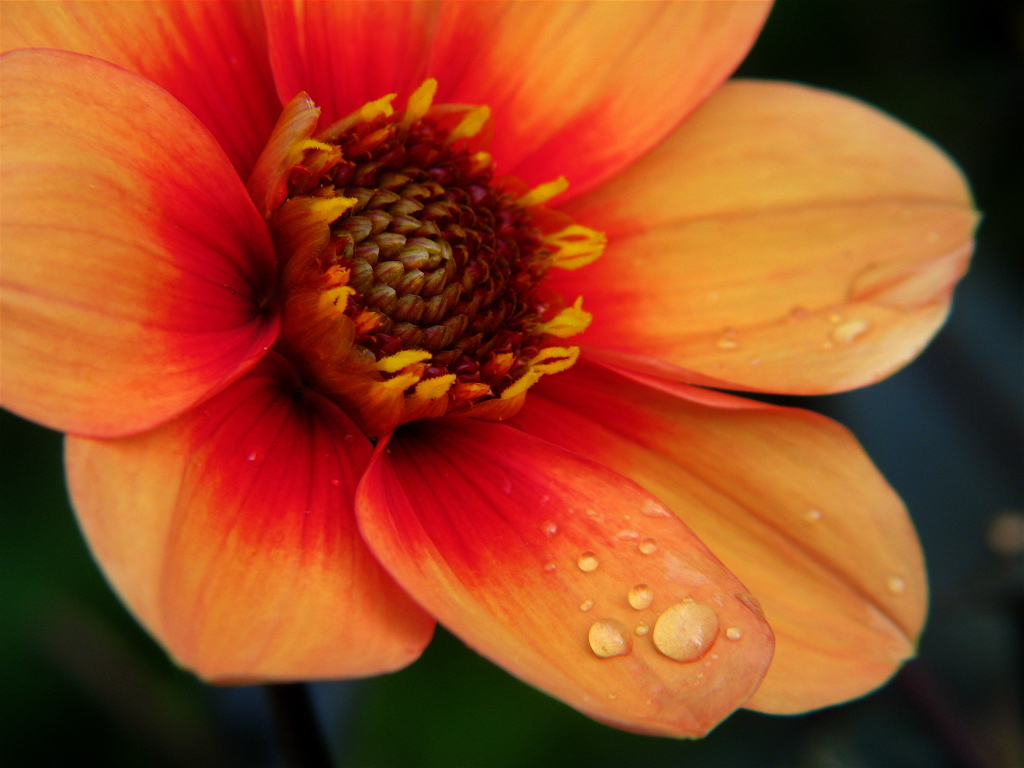
\includegraphics[scale=0.3]{figures/flower.jpg}
	\caption[Background segmentation]{
		The human visual system has no issue interpreting the subtle changes in translucency and shading in this photograph and segmenting the object from its background.
	}
	\label{flower}
\end{figure}

\section{Computer Vision}

As humans, we perceive the tridimensional structure of the world around us with apparent ease. Think of how vivid the tridimensional perception is when one looks at a vase of flowers sitting on the table. You can tell the shape and translucency of each petal through the subtle patterns of light and shading that play across its surface. One can easily segment
each flower from the background of the scene (see \autoref{flower}).

Looking at a framed group portrait, you can effortlessly for example count all of the people and even guess their emotions from their facial appearance. Perceptual psychologists have spent decades trying to understand how the visual system works and, even though they can find optical illusions to tease apart some of its principles (see \autoref{optical_illusion}), a solution to the complete puzzle remains elusive.

\begin{figure}[h]
	\centering
	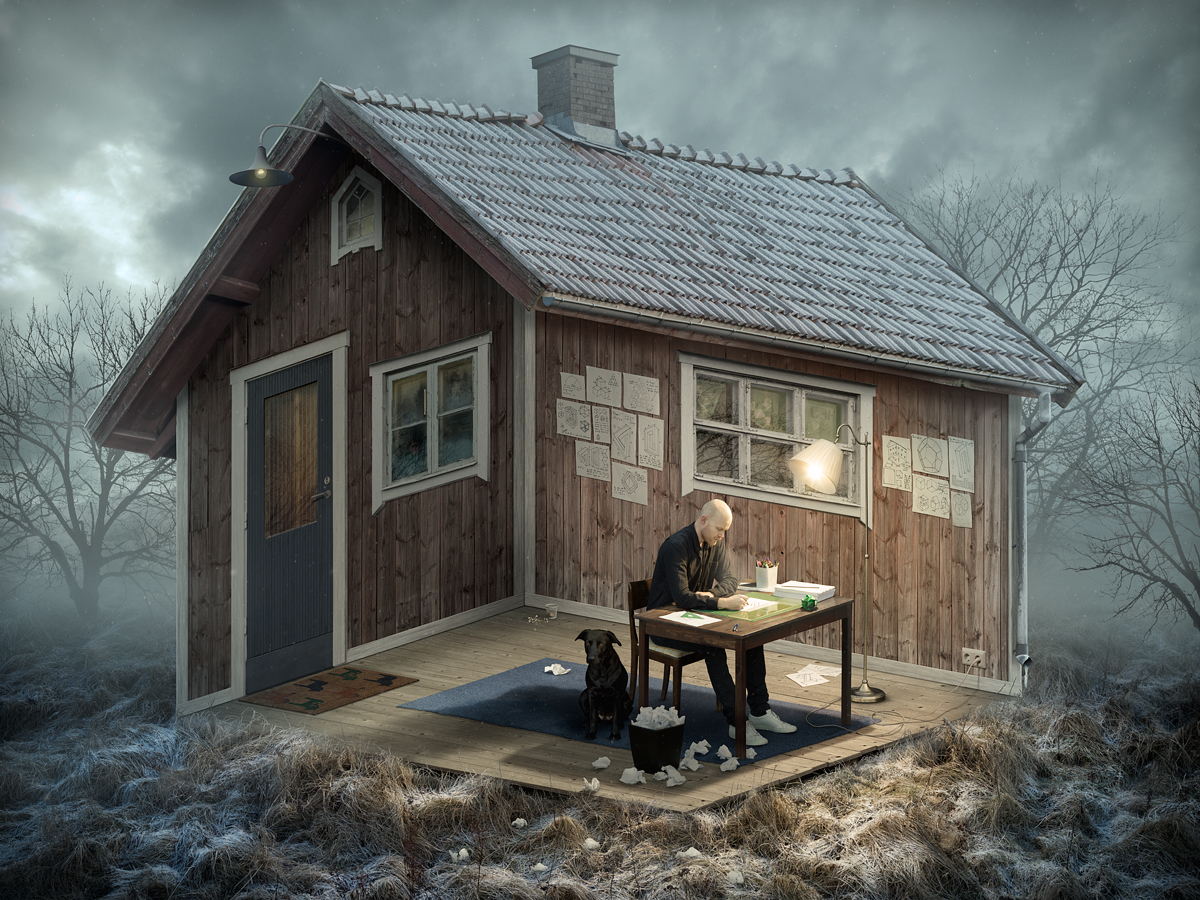
\includegraphics[scale=0.3]{figures/optical_illusion.jpg}
	\caption[Optical illusion]{
		 This work by Eric Johansson is composed of optical illusions that use highly creative pieces that render manipulations of perspective to make the viewer see a perplexed set of images. 
	}
	\label{optical_illusion}
\end{figure}

In areas, such as rendering a still scene composed of everyday objects or animating extinct creatures such as dinosaurs, the illusion of reality is almost perfect. In computer vision, we are trying to do the opposite, i.e., to describe the world that we see in one or a sequence of images and to reconstruct its properties, such as shape, illumination, and color distributions. It is incredible that humans and animals do this so effortlessly, while computer vision algorithms are so error prone.

Applications range from tasks such as industrial machine vision systems which, say, inspect bottles speeding by on a production line, to research into artificial intelligence and computers or robots that can comprehend the world around them. In many computer vision applications, the computers are preprogrammed to solve a certain task, but methods based on learning are now becoming more common. Examples of applications of computer vision include systems for:

\begin{itemize}
\item Process control.
\item Navigation.
\item Event detection. 
\item Information organization.
\item Object or environment modeling.
\item Interaction.
\item Automatic inspection.
\item Etc.
\end{itemize}

Each of the application areas described above employ a range of computer vision tasks; more or less well-defined measurement problems or processing workloads, which can be solved using a variety of methods. Some examples of typical computer vision tasks are presented below:

\begin{itemize}
\item \textbf{Recognition:} the classical problem in computer vision, image processing, and machine vision is that of determining whether or not the image data contains some specific object, feature, or activity.
\item \textbf{Motion analysis:} several tasks relate to motion estimation where an image sequence is processed to produce an estimate of the velocity either at each points in the image or in the 3D scene, or even of the camera that produces the images.
\item \textbf{Scene reconstruction:} Given one or (typically) more images of a scene, or a video, scene reconstruction aims at computing a 3D model of the scene.
\item \textbf{Image restoration:} The aim of image restoration is the removal of noise (sensor noise, motion blur, etc.) from images.
\end{itemize}

\begin{figure}
  \centering
  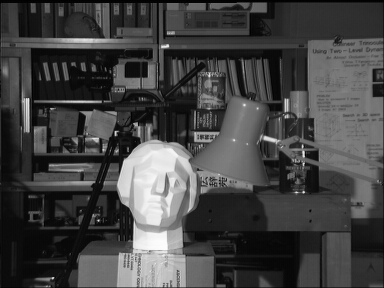
\includegraphics[width=0.475\textwidth]{figures/tsukuba_l.png} \quad
  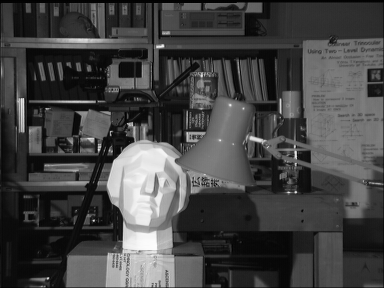
\includegraphics[width=0.475\textwidth]{figures/tsukuba_r.png}
  \caption{Example of stereoscopic images employed in scene reconstruction.}\label{tsukuba_ims}
\end{figure}

Our main interest in this project is \emph{scene reconstruction} from one or more pairs of images (see \autoref{tsukuba_ims}), specifically with stills obtained using stereo vision techniques. This images can be processed to obtain a depth estimation of the scene, once it is known, we have a 3D model of said scene.  

\subsection{Stereo Vision}

Any technique that is capable of collecting 3D information and creating the illusion of depth in an image, is considered stereoscopic vision or tridimensional (3D) vision. Our vision is stereoscopic by nature, being able to perceive the sensation of depth, distance, etc. This is achieved thanks to the horizontal separation between our eyes, leading to the processing of the differences between the perceived images of the visual system by our brain. 

Computer stereo vision is the extraction of 3D information from digital images, such as obtained by a CCD camera. Artificial systems for stereoscopic vision for the obtaining of 3D information in multiple applications, have been employed for several decades. The main problem that these systems tackle; is the determination of the correspondence between the pixels that come from the same point in the image pairs of the tridimensional scene. By comparing information about a scene from two vantage points, 3D data can be extracted by examination of the relative positions of objects in the two panels (see \autoref{stereo_vision}). %Wiki: https://en.wikipedia.org/wiki/Computer_stereo_vision

\begin{figure}[h]
	\centering
	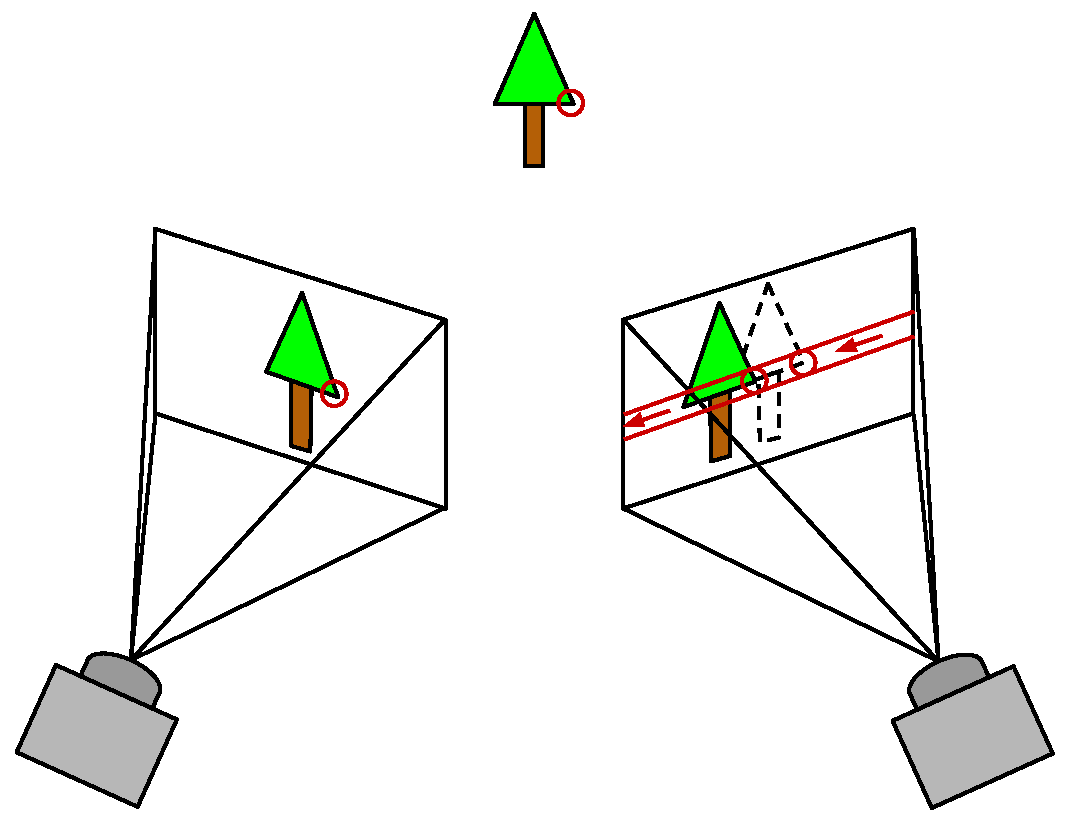
\includegraphics[scale=0.3]{figures/stereo_vision.pdf}
	\caption[Stereo vision]{
		 Diagram describing relationship of image displacement to depth with stereoscopic images, assuming flat co-planar images. 
	}
	\label{stereo_vision}
\end{figure}

\subsection{Stereo Correspondence}

Given two or more images of the same 3D scene, taken from different vantage points, the correspondence problem refers to the task of finding a set of points in one image which can be identified as the same points in another image. To achieve this, points or features in one image are matched with the corresponding points or features in another image. The images can be taken from a different point of view, not at the same time, or with objects in general motion relative to the cameras.

From the earliest forays into visual perception, it was known that we depth is perceived based on the differences in appearance between the left and right eye. As a simple test, hold your finger vertically in front of your eyes and close each eye at a time. You will notice that the finger jumps left and right, relative to the background of the image. The same effect is visible in the image pair shown in \autoref{tsukuba_depth}, in which the foreground objects shift left and right with respect to the background.

Stereo Matching is the process of employing two or more images and estimating a 3D model of the scene by finding matching areas of interest in the images and converting their 2D positions into 3D depths. This tackles the question of how to build a better 3D model, e.g., a sparse or dense depth map that assigns relative depths to pixels in the input images (see \autoref{tsukuba_depth}).

\begin{figure}[h]
  \centering
  \subfigure[Tsukuba left]{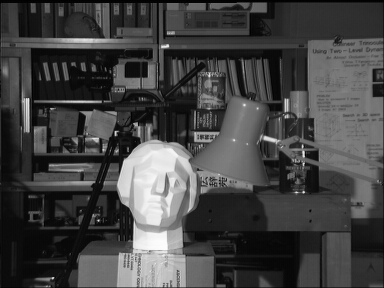
\includegraphics[width=0.29\textwidth]{figures/tsukuba_l.png}} \hfill
  \subfigure[Tsukuba right]{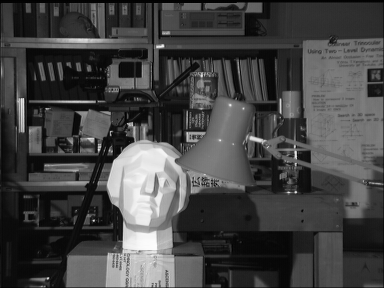
\includegraphics[width=0.29\textwidth]{figures/tsukuba_r.png}}\hfill
  \subfigure[Depth map]{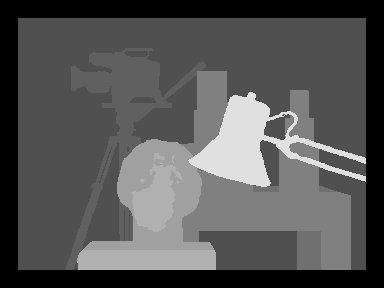
\includegraphics[width=0.29\textwidth]{figures/tsukuba_o_d.jpg}}
  \caption[Stereo reconstruction]{Stereo reconstruction techniques can convert (\textbf{a}-\textbf{b}) a pair of images, into (\textbf{c}) a depth map.}
  \label{tsukuba_depth}
\end{figure}

There are two main types of techniques for stereo matching:

\begin{itemize}
\item \textbf{Sparse} algorithms
\item \textbf{Dense} algorithms
\end{itemize}

Early stereo matching techniques were feature-based, i.e., they first extracted a set of potentially matchable image locations, using either interest operators or edge detectors, and then searched for matching locations in other images using a patch-based metric \cite{bolles1993jisct,hsieh1992performance}. This limitations to sparse correspondences were in part due to computational resource limitations, but also were driven by a need to limit the answers produced by algorithms to matches with high confidence.

While sparse matching algorithms are still used on occasion, most stereo matching algorithms today focus on dense correspondence. This came to be since it is required for applications, such as image-based rendering or modeling. This problem is more difficult than sparse correspondence, since inferring depth values in regions with similar textures requires making a certain amount of inferences.

After carefully studying multiple algorithms to achieve our goal, we have chosen Block Matching. This is not one of the algorithms with the highest precision, but we believe it can be highly parallel and fits our requirement of real-time processing of video images.

\begin{algorithm}[h]
	\DontPrintSemicolon
	\caption{Block Matching algorithm}
	\label{BMalgorithm}
	\KwIn{$left$, $right$, $aggregationdim$, $maxdisparity$}
	\KwOut{$depthmap$}
	\BlankLine
	$radius \leftarrow aggregationdim/2$\;
	\For{$x\leftarrow 0$ \KwTo $width$}{
		\For{$y\leftarrow 0$ \KwTo $height$}{
			$offsetx \leftarrow x - radius$\;
			$offsety \leftarrow y - radius$\;
			$sum \leftarrow 0$\;
			$bestsum \leftarrow -1$\;
			\For{$d\leftarrow 0$ \KwTo $maxdisparity$}{
				\For{$i\leftarrow offsetx$ \KwTo $aggregationdim + offsetx$}{	
					\For{$j\leftarrow offsety$ \KwTo $aggregationdim + offsety$}{
						$sum \leftarrow sum + \left | left[i * width + j] - left[i * width + j - d] \right |$\;
					}
				}
				\If{$sum < bestsum$}{
					$bestsum \leftarrow sum$\;
					$bestd \leftarrow d$\;
				}
				$sum \leftarrow 0$\;			
			}
			$depthmap[y * width + x] \leftarrow bestd$\;
		}
	}
\end{algorithm}

\subsection{Block Matching}

The chosen algorithm follows a similar structure to the following publication \cite{scharstein2002taxonomy}. With stereo cameras, objects in the field of view of these will appear at slightly different locations within the two images due to the cameras varying perspectives of the same scene. A standard method for calculating the disparity map is to use Block Matching, essentially, we will be taking a small region of pixels in the right image, and searching for the closest matching region of pixels in the left image. The structure and pseudo code of the implemented algorithm can be seen in \autoref{BMalgorithm}.

Correlation based matching typically produces dense depth maps by calculating the disparity at each pixel within a neighborhood. This is achieved by taking a square window of certain size around the pixel of interest in the reference image and finding the homologous pixel within the window in the target image, while moving along the corresponding scanline. The goal is to find the corresponding (correlated) pixel within a certain disparity range $d$ that minimizes the associated error and maximizes the similarity (see \autoref{window_search}).

%TODO source?
\begin{figure}[h]
	\centering
	\subfigure[Left image]{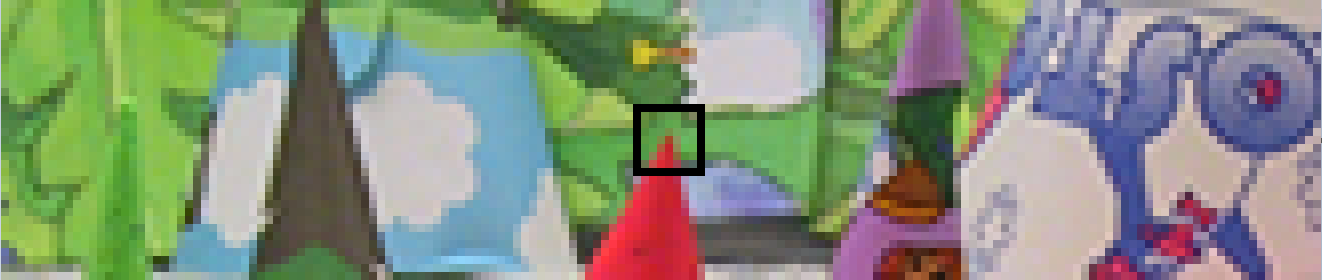
\includegraphics[scale=0.4]{figures/left_wsearch_crop.png}}
	\subfigure[Right image search]{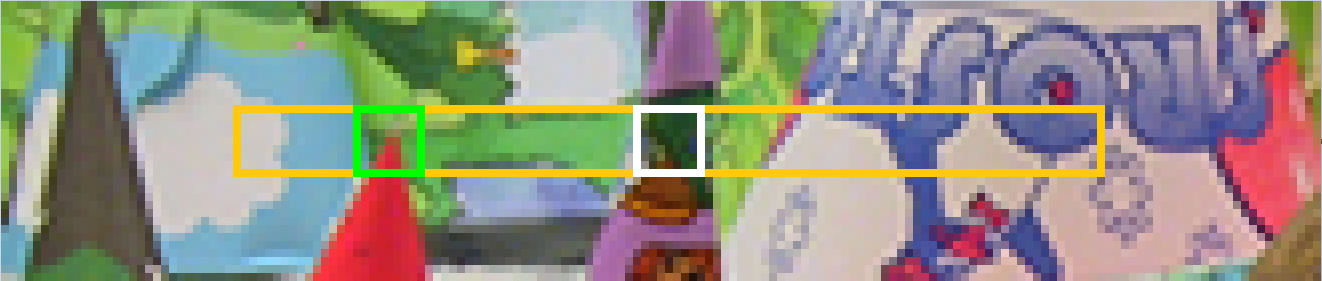
\includegraphics[scale=0.4]{figures/right_wsearch_crop.png}}
	\caption[Stereo vision]{
		 Diagram describing relationship of image displacement to depth with stereoscopic images, assuming flat co-planar images. 
	}
	\label{window_search}
\end{figure}

The most relevant part in this algorithm, is the comparison of the pixel windows between the left and right images. In our implementation we have implemented two approaches. The first, uses the following equation to calculate the \textit{Sum of Absolute Differences} (SAD) between pixels:

\begin{equation}\sum_{i,j\in W} \left | I_{l}(i,j) - I_{r}(i,j) \right |\end{equation}

Being $W$ the aggregation window dimension, $I_{l}$ the left image and $I_{r}$ the right image. The second uses a \textit{Sum of Squared Differences} (SSD) to achieve the same objective as we can observe in the next equation:

\begin{equation}\sum_{i,j\in W}  (I_{l}(i,j) - I_{r}(i,j))^2\end{equation}

Being $W$ the search window dimension, $I_{l}$ the left image and $I_{r}$ the right image. One of these calculations is repeated for pixel windows in the right image at a distance $d\in[0,disparity_{max}]$.

In short, the correspondence process involves the computation of the similarity measure for each disparity value, followed by an aggregation and optimization step. Since these steps consume a lot of processing power but can be computed in parallel, there are significant speed-performance advantages to be had in optimizing the matching algorithm.

\section{GPGPU}

\textit{General-purpose computing on graphics processing units} or GPGPU, is the use of a graphics processing unit (GPU), which typically handles computation only for computer graphics workloads, to perform calculations in applications traditionally handled by the central processing unit (CPU) \cite{fung2002mediated}. One can parallelize tasks even further using multiple graphics cards in one computer, or large numbers of graphics chips \cite{fung2004using}.

\subsection{Architecture}

Essentially, a GPGPU pipeline swaps data between one or more GPUs and CPUs and analyzes it as if it were in image or other graphic form. Because video cards can operate on 3D geometry and graphical data at speeds way faster than a traditional CPU, migrating data into graphical form and then using the GPU to process it and analyze it, can result in profound speed gains.

In a traditional \textbf{CPU architecture}, the CPU is able to access a large, general-purpose memory bank, called Random Access Memory (RAM) as is visually seen in \autoref{cpu_arch}.

\begin{figure}[h]
	\centering
	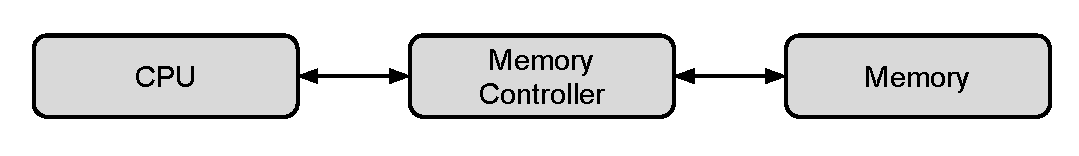
\includegraphics[scale=0.7]{figures/cpu_arch.pdf}
	\caption[CPU Architecture]{
	 Diagram describing a simplified CPU architecture. 
	}
	\label{cpu_arch}
\end{figure}

Nowadays, the CPU often contains more than one core, making CPUs capable of more than one task at a time.  This makes modern CPUs much faster than their single core, scalar predecessors.

In contrast, a \textbf{GPGPU architecture} uses \textit{Shared-Memory Multiprocessors} (SMP), these are a are a set of processors that all have their own local memory. These memory banks are shared within a thread group, but not between more than one of these groups.  However, each compute unit also has access to a global memory bank, which is shared between all processors.

\begin{figure}[h]
	\centering
	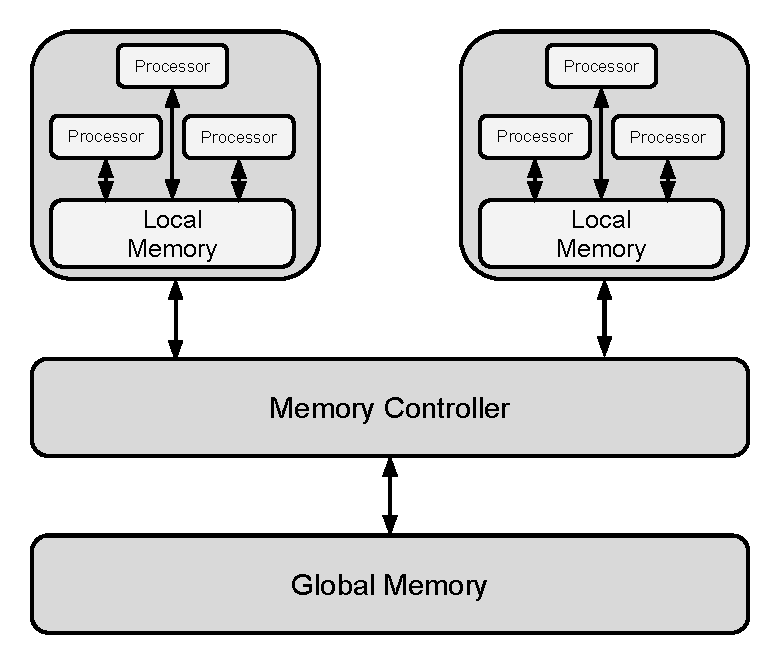
\includegraphics[scale=0.6]{figures/gpu_arch.pdf}
	\caption[GPU Architecture]{
	 Diagram showing a simplified SMP architecture. 
	}
	\label{gpu_arch}
\end{figure}

This is the parallel architecture that NVIDIA and AMD both use in their GPUs. Likewise, it is also the model enforced in the OpenCL and CUDA specification.

\subsection{OpenCL}

\textit{Open Computing Language} (OpenCL) is a framework for writing programs that make use of heterogeneous platforms consisting of CPUs, GPUs, digital signal processors (DSPs), field-programmable gate arrays (FPGAs) and other processors. OpenCL provides parallel computing using task-based and data-based parallelism. In addition, it is also an open standard maintained by the non-profit technology consortium Khronos Group \footnote{https://www.khronos.org/}.

OpenCL interprets a computing system as a number of heterogeneous compute devices, which might be CPUs or accelerators such as graphics processing units, attached to a host processor (a CPU). It defines a C-like language for writing programs, called kernels, that are later executed on the compute devices. A single compute device typically consists of several compute units, which in turn comprise multiple \textit{processing elements} (PEs). 

A single kernel execution may run on all or many of the PEs in parallel. How a compute device is subdivided into compute units and PEs depends on vendor criteria; a compute unit can be thought of as a CPU core, but the notion of core is hard to define across all the types of devices supported by OpenCL and the number of compute units may not correspond to the number of cores that the vendor can advertise.

\begin{figure}[h]
	\centering
	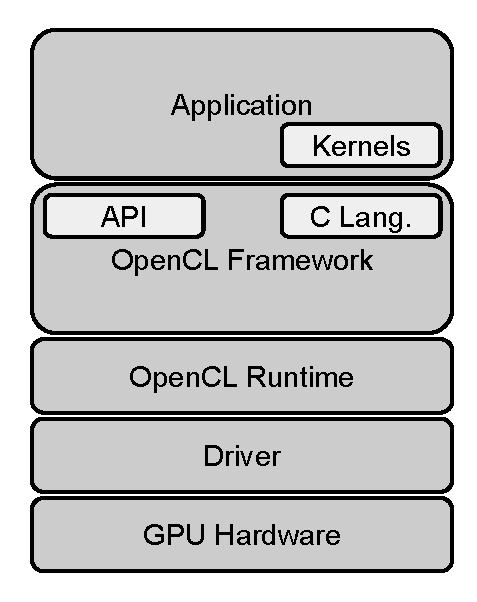
\includegraphics[scale=0.7]{figures/opencl_arch.pdf}
	\caption[OpenCL Architecture]{
	 Diagram showing the simplified OpenCL architecture. 
	}
	\label{opencl_arch}
\end{figure}

In addition to its this kernel programming language, OpenCL defines an \textit{application programming interface} (API) that allows normal programs running on the host to launch kernels on the compute devices and manage device memory, which is (at least conceptually) separate from host memory. Programs in the OpenCL language are intended to be compiled at run-time, so that applications that use OpenCL are portable between implementations for various host devices (see \autoref{opencl_arch}).

OpenCL defines a four-level memory hierarchy for the compute device:

\begin{itemize}
\item \textbf{Global memory:} Shared by all processing elements, but has high access latency.
\item \textbf{Read-only memory:} Smaller, low latency, writable by the host CPU but not the compute devices.
\item \textbf{Local memory:} Shared by a group of processing elements.
\item \textbf{Private memory:} Per-element private memory (registers).
\end{itemize}

\subsection{CUDA}

\textit{Compute Unified Device Architecture} (CUDA) is a parallel computing platform and application programming interface (API) model created by NVIDIA. It allows software developers to use CUDA-enabled GPUs for general purpose processing. The CUDA platform is a software layer that gives direct access to the virtual instruction set and parallel computational elements of GPUs.

In contrast with OpenCL, this is a proprietary framework and is not compatible with such a varied array of devices, CUDA is only compatible with NVIDIA GPUs. It is compatible with programming languages such as C, \CC and Fortran. This makes it easier for specialists in parallel programming to utilize GPU resources, as opposed to previous API solutions like Direct3D and OpenGL, which required advanced skills in graphics programming.

\begin{figure}[h]
	\centering
	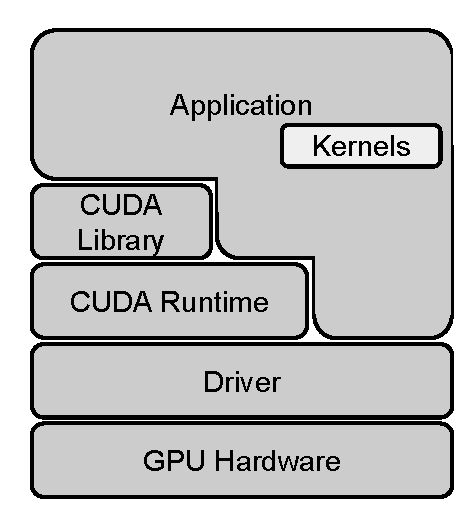
\includegraphics[scale=0.7]{figures/cuda_arch.pdf}
	\caption[CUDA Architecture]{
	 Diagram showing the simplified CUDA architecture. 
	}
	\label{CUDA_arch}
\end{figure}

Another difference between OpenCL and CUDA is how applications are compiled. In OpenCL kernels are compiled ad-hoc with the OpenCL framework, while in CUDA we will use a custom copiler called NVCC to compile the complete application or the parts that contain CUDA code. The CUDA architecture is built around a scalable array of multiprocessors, each one of them having several scalar processors, one multi-threading unit, and a shared memory chip. The multiprocessors are able to create, manage, and execute parallel threads, with a small overhead. The threads are grouped in blocks, which are executed in a single multiprocessor, and the blocks are grouped into grids. When a CUDA program calls a grid to be executed in the GPU, each one of the blocks in the grid is numbered and distributed to an available multiprocessor. When a multiprocessor receives a block to execute, it splits the threads in warps, a set of 32 consecutive threads. Each warp executes a single instruction at a time, so the best efficiency is achieved when the 32 threads in the warp executes the same instruction. Each time that a block finishes its execution, a new block is assigned to the available multiprocessor. 

CUDA defines a similar memory hierarchy for compute devices:

\begin{itemize}
\item \textbf{Global memory:} Shared by all processing elements, but has high access latency.
\item \textbf{Read-only memory:} Smaller, low latency, writable by the host CPU but not the compute devices.
\item \textbf{Shared memory:} Shared by a block of threads.
\item \textbf{Local memory:} Per-thread local memory.
\item \textbf{Register memory:} Per-thread registers.
\end{itemize}